\documentclass[tikz,border=2]{standalone}
%% \usepackage{amsfonts}
\usepackage{lmodern} % enhanced version of computer modern
\usepackage[T1]{fontenc} % for hyphenated characters
\usepackage{amssymb}
\usepackage{amsmath}
\usepackage{amsthm}
%
\usetikzlibrary{decorations.pathreplacing,shadows,arrows,shapes,positioning,calc,backgrounds,fit}
\newcommand{\mA}{\mathcal{A}}
\newcommand{\mB}{\mathcal{B}}
\newcommand{\mC}{\mathcal{C}}
\newcommand{\mI}{\mathcal{I}}
\newcommand{\mN}{\mathcal{N}}
\newcommand{\mP}{\mathcal{P}}
\newcommand{\mR}{\mathcal{R}}
\newcommand{\mS}{\mathcal{S}}
\newcommand{\mY}{\mathcal{Y}}
% Define the layers to draw the diagram
%
\begin{document}
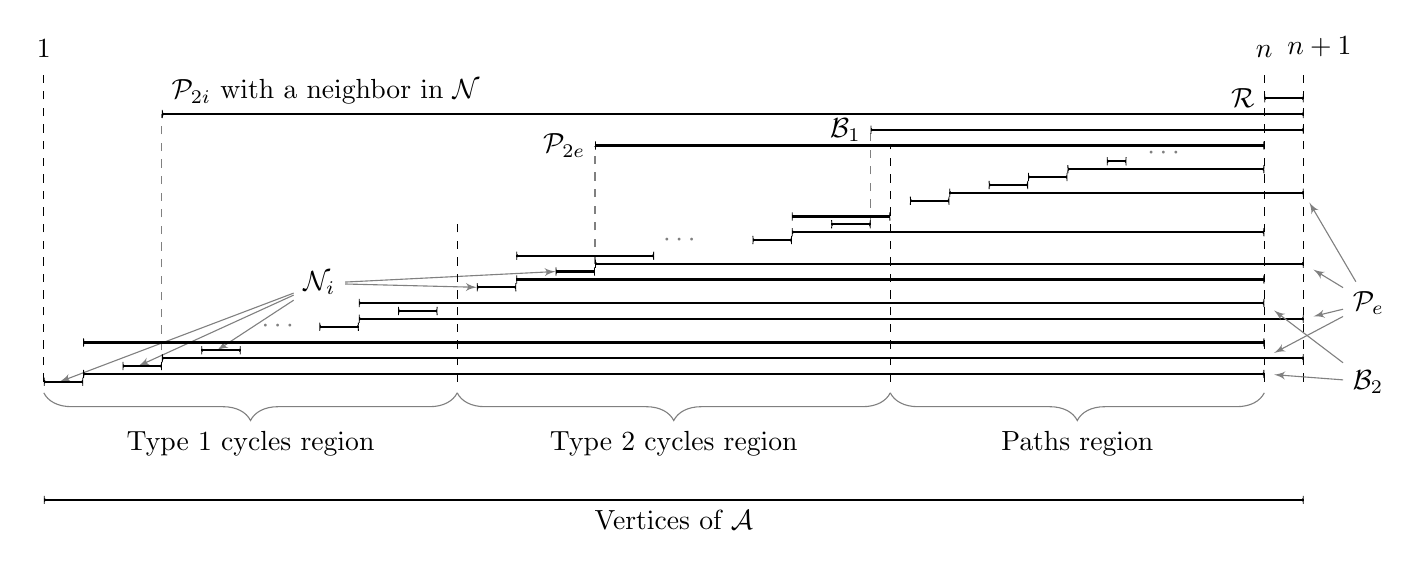
\begin{tikzpicture}
[node distance=1cm,
interval/.style={thick,>=serif cm,rounded corners=1.24pt},
uint/.style={shape=rectangle,draw=black,inner sep=.5pt,fill},
dedge/.style={gray,>=latex', shorten >=.0pt, shorten <=.0pt},
myedge/.style={thick}]
%%
% boundaries
%%
\node (1) at (.5,0){};
\node (n) at (16,0){};
\node (np1) at (16.5,0){};
\draw[dashed] (1)+(0,-1.5) -- +(0,2.5) node[above] {$1$};
\draw[dashed] (n)+(0,-1.5) -- +(0,2.5) node[above] {$n$};
\draw[dashed] (np1)+(0,-1.5) -- +(0,2.5) node[above,xshift=.2cm] {$n+1$};
%%
% B2PeN
%%
%%
% Type 1
%%
\node at (4,-.25) (Ni) {$\mN_i$};
\path 
(Ni) edge[dedge,->] (.7,-1.5)
(Ni) edge[dedge,->] (1.7,-1.3)
(Ni) edge[dedge,->] (2.7,-1.1)
(Ni) edge[dedge,->] (6,-.3)
(Ni) edge[dedge,->] (7,-.1);
\path[yshift=-1.5cm] 
(.5,0) edge[interval,<->] +(.5,0)
(1,.1) edge[interval,<->] (n|-0,.1)
node (b21) at (n|-0,.1) {} 
(1.5,.2) edge[interval,<->] +(.5,0)
node (T1N1) at (2,0) {} 
(2,.3) edge[interval,<->] (np1|-0,.3) 
node (pe1) at (n|-0,.3) {} 
(2.5,.4) edge[interval,<->] +(.5,0)
(1,.5) edge[interval,<->] (n|-0,.5);
\path[yshift=-1.5cm]
(3.5,.7) node[gray] {$\cdots$}
(4,.7) edge[interval,<->] +(.5,0)
(4.5,.8) edge[interval,<->] (np1|-0,.8)
node (pe2) at (np1|-0,.8) {} 
++(.5,.1) edge[interval,<->] +(.5,0)
(4.5,1) edge[interval,<->] (n|-0,1)
node (b22) at (n|-0,1) {};
%%
\draw[dashed,yshift=-1cm] (5.75,-.5) -- +(0,2) node[above right] {};
\draw [gray,decorate,decoration={brace,amplitude=10pt,mirror,raise=4pt},yshift=0pt]
(1|-0,-1.5) -- +(5.25,0) node [midway,below,yshift=-.5cm,black] {Type 1 cycles
region};
%%
% Type 2
%%
\path[yshift=-0.3cm,xshift=6cm]
(0,0) edge[interval,<->] +(.5,0)
(.5,.1) edge[interval,<->] (n|-0,.1)
(1,.2) edge[interval,<->] +(.5,0) 
node (T2N1) at (1.5,0) {} 
(1.5,.3) edge[interval,<->] (np1|-0,.3)
node (pe3) at (np1|-0,.3) {} 
(.5,.4) edge[interval,<->] (2.25,.4)
(2.6,.6) node[gray] {$\cdots$};
\path[yshift=0.3cm,xshift=9.5cm]
(0,0) edge[interval,<->] +(.5,0)
(.5,.1) edge[interval,<->] (n|-0,.1)
(1,.2) edge[interval,<->] +(.5,0)
node (T2N2) at (1.5,0) {} 
(.5,.3) edge[interval,<->] (1.75,.3);
%%
\draw[dashed,yshift=0cm] (11.25,-1.5) -- +(0,3) node[above right] {};
\draw [gray,decorate,decoration={brace,amplitude=10pt,mirror,raise=4pt},yshift=0pt]
(5.75,-1.5) -- (11.25,-1.5) node [midway,below,yshift=-.5cm,black] {Type 2 cycles
region};
%%
% Paths
%%
\path[yshift=.8cm,xshift=11.5cm]
(0,0) edge[interval,<->] node (ne1){} +(.5,0)
(.5,.1) edge[interval,<->] (np1|-0,.1)
node (pe4) at (np1|-0,.1) {} 
(1,.2) edge[interval,<->] +(.5,0)
(1.5,.3) edge[interval,<->] +(.5,0) 
(2,.4) edge[interval,<->] (n|-0,.4) 
(2.5,.5) edge[interval,<->] +(.25,0) 
(3.25,.6) node[gray] {$\cdots$};
%%
\draw [gray,decorate,decoration={brace,amplitude=10pt,mirror,raise=4pt},yshift=0pt]
(11.25,-1.5) -- (n|-0,-1.5) node [midway,below,yshift=-.5cm,black] {Paths region};
%%
% B1, P2e, R and P2i
%%
\path[yshift=1.5cm]
(T2N1|-0,0) edge[interval,<->] (n|-0,0) node [left] {$\mP_{2e}$}
(T2N2|-0,.2) edge[interval,<->] (np1|-0,.2) node [left] {$\mB_1$}
(T1N1|-0,.4) edge[interval,<->] (np1|-0,.4) node [above right] {$\mP_{2i}$
with a neighbor in $\mN$}
(n|-0,.6) edge[interval,<->] (np1|-0,.6) node [left] {$\mR$};
%% connecting vertical lines
\begin{pgfonlayer}{background}
\path
(T2N1|-0,0) edge[dashed,gray] (T2N1|-0,1.5)
(T2N2|-0,0.5) edge[dashed,gray] (T2N2|-0,1.7)
(T1N1|-0,-1.1) edge[dashed,gray] (T1N1|-0,1.9);
\end{pgfonlayer}
%%(np1|-0,.5) node[uint] (p2i) {};
%%
% A
%%
\path[yshift=-3cm]
(1|-0,0) edge[interval,<->] node [midway,below] {Vertices of $\mA$} (np1|-0,0);
%%
% P2e labeling
%%
\node[right,xshift=.5cm] (pe) at (np1|-0,-.5) {$\mP_{e}$};
\path
(pe) edge[dedge,->] (pe1)
(pe) edge[dedge,->] (pe2)
(pe) edge[dedge,->] (pe3)
(pe) edge[dedge,->] (pe4);
%%
% B2 labeling
%%
\node[right,xshift=.5cm] (b2) at (np1|-0,-1.5) {$\mB_2$};
\path
(b2) edge[dedge,->] (b21)
(b2) edge[dedge,->] (b22);
\end{tikzpicture}
{}
\end{document}
